\section{Description Of Research Tasks, Progress, And Plans}
\label{sec:research}

{\small\color{red}
\begin{itemize}
\item 12 pages max
    \item Include an Executive Summary of the progress made since September 2019 toward
meeting its strategic objectives, making clear how the accomplishments described in detail in Section 6 below fit together as part of a synergistic research program.
\begin{enumerate}
    \item Specific research objectives associated with each task
    \item Research progress for each task since the start of the project
    \item Integration of research activities across tasks
    \item Research planned for the balance of the award period (through September 2023).
\end{enumerate}
\item In the descriptions of the tasks and their integration, the need for a collaborative, synergistic approach involving several investigators should be clearly established. The role and intellectual contribution of each senior investigator should be clear to the reviewer, and the availability of the resources necessary to accomplish the research objectives should be evident. Approximately 70\% of this section should be dedicated to research progress to date and 30\% to planned research.
    \item \textcolor{red}{Review criteria for Scientific and/or Technical Merit of the Proposed Research:}
    \begin{itemize}
        \item \textcolor{red}{What new capability/functionality will the proposed software provide to the materials research community? How will the research plan attain the 4-year research and software/data goals?}
        \item \textcolor{red}{Comment on the novelty and scientific value of the proposed research. }
        \item \textcolor{red}{How widespread would be the interest in the software within the materials research community?}
        \item \textcolor{red}{How does the proposed work compare with other efforts in its field, both in terms of scientific and/or technical merit and originality?}
        \item \textcolor{red}{Comment on the progress and impact for the current award period.}
    \end{itemize}

\end{itemize}
}
{\color{green}
Note to ourselves:
\begin{itemize}
    \item TB-INQ integration in future: forced oscillation? any idea? Keep in mind: non perturbative aspect is very important.
    \item k-points and non-orthgonal cell
    \item User defined operation for external collaborator? How to balance with performance?
    \item How to expand user base need to be spelled out: Online tutorial by Xavier in late summer, ESW, TMF users meeting (Liang gave us material), SLAC (name?) workshop, US-Africa collaboration (?)
    \item CCMS to expand collaboration: two summer student from Andre and ? with Alfredo and Kejun from Yuan with Tadashi. Perhaps, get theirs support information and relevant research area to make it more convincing and conpelling.
\end{itemize}

}
\clearpage

\section{Progress and Accomplishments to date} 
As outlined above, the primary strategic objective of the NPNEQ team during the first 18 months of the funding period was the development of a scalable and extensible DFT/TDDFT platform that is fully compatible with existing petascale and medium-term exascale hybrid CPU-GPU architectures. This objective was achieved with the recent release of the INQ platform. In parallel however, the team also pursued collaborative research efforts leading to science outcomes in the area of ultrafast materials science using existing tools and methods some of which will be incorporated into the larger INQ ecosystem of codes in future. In the following we provide a summary of both the software development and scientific research efforts within NPNEQ.   
\subsection{Code Development}
\subsubsection{The INQ DFT/TDDFT platform} (4 pages total)
\paragraph{General features and design}
1-1.5 pages including figures
\paragraph{GPU-MPI functionality and scaling}
1-1.5 pages including figures
\paragraph{Validation of results}
1 page including figures

Mention stopping, hook to Future work

\subsubsection{Sangeeta's tight binding code}
1-1.5 pages Description of capabilities and code improvements carried out under NPNEQ.

\subsection{Collaborative science}
\textcolor{red}{Descriptions of type-A projects.}

\subsubsection{Role of nonequilibrium spin-phonon coupling in enhancing bulk photovoltaic effect }
During the project period, our work on the materials system of \(\mathrm{Pr_xCa_{1-x}MnO_3}\) has resulted in the discovery of a new way to enhance the bulk photovoltaic effect by optically induced phase transitions. 
These results, currently under review, are reported in the preprint Ref.~\cite{Rajpurohit2021}. 
Our study provides a unified picture of the photocurrent generation and its evolution through real-time simulations, and will have a significant impact in field of the bulk photovoltaic effect (BPVE) where understanding, predicting, and ultimately controlling the photovoltaic behavior remains a challenge.
We show theoretically that this strongly correlated oxide perovskite displays strong photocurrent enhancement when it is driven into a hidden magnetic phase transition.
This phenomenon is highly non-perturbative, and lies outside the perturbative paradigm of shift and ballistic currents used in this field. 
The maximum photoresponsivity obtained is almost an order of magnitude higher than that reported for other transition metal oxides such as \(\mathrm{BiFeO_3}\) and \(\mathrm{BaTiO_3}\).

\begin{figure}[ht]
    \centering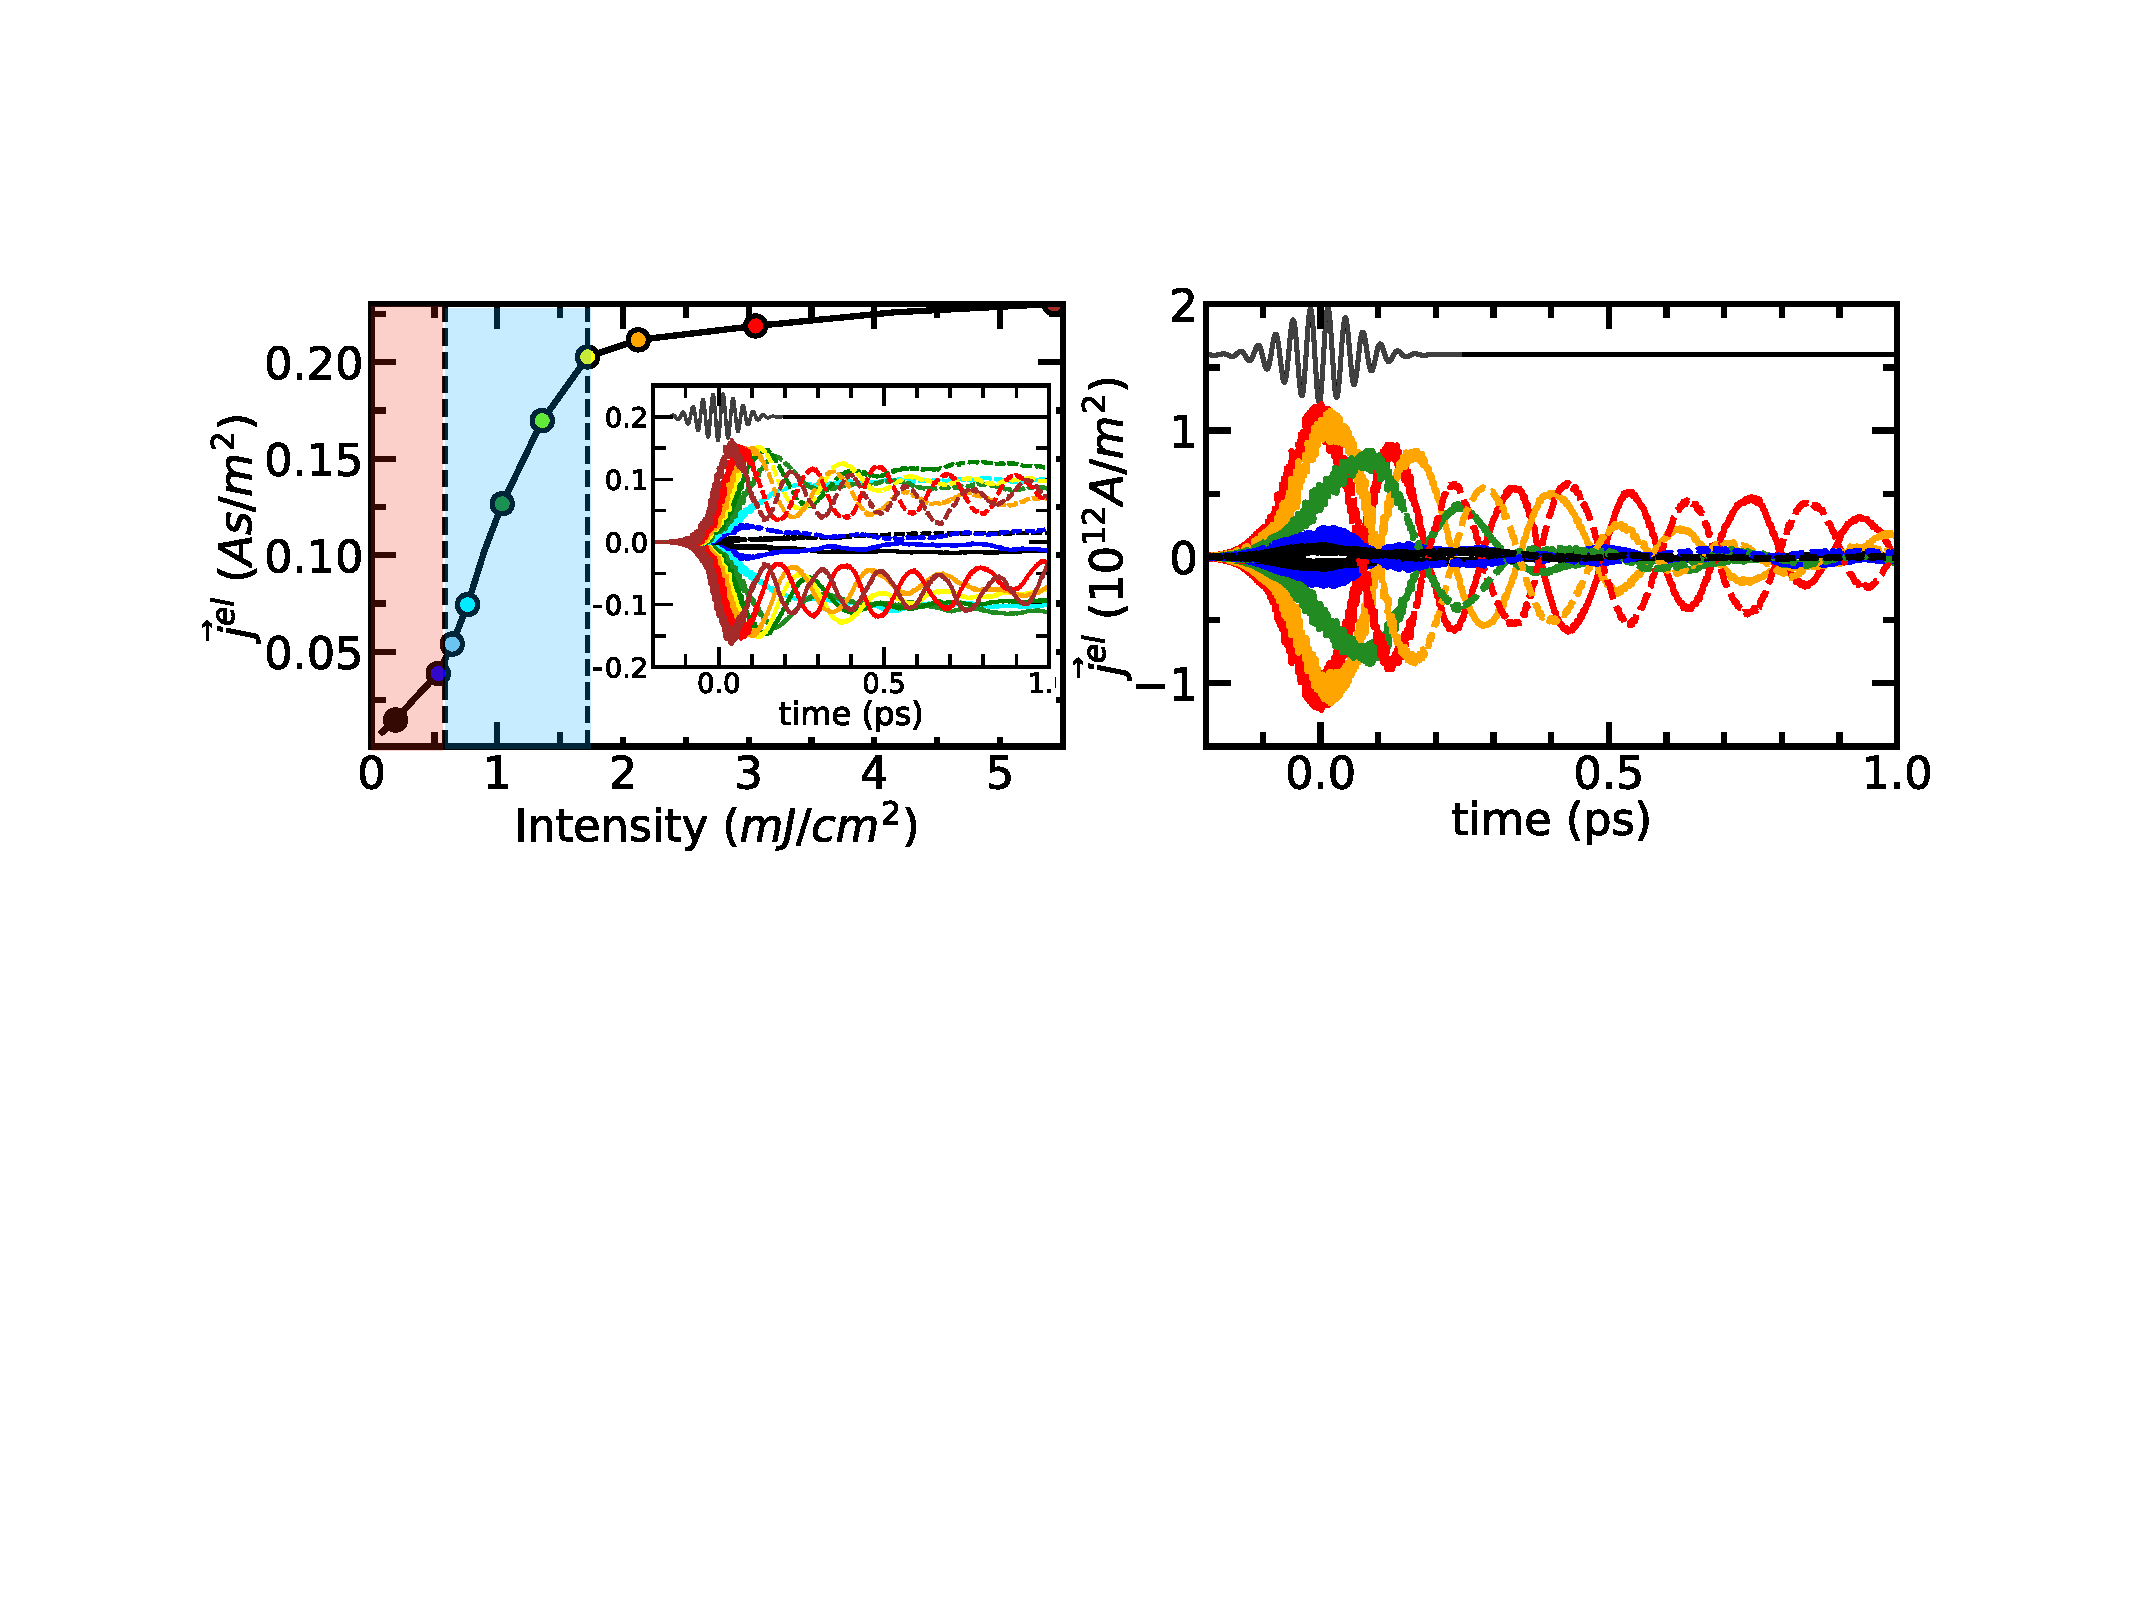
\includegraphics[width=1.0\linewidth]{figures/photocurrent_old}
    \caption{
        Simulated photocurrent of \(\mathrm{Pr_xCa_{1-x}MnO_3}\), as a function of light intensity and time after excitation. 
        Rapid enhancement of photocurrent (left) in indicative of a nonperturbative process beyond the frameworks of previously studied shift and ballistic current theories.
    }
    \label{fig:PCMO}
\end{figure}

To study this effect, we use a methodology based on real-time simulations of a first-principles based Hubbard model which treats all the relevant degrees of freedom, namely charge, spin, orbital and lattice, explicitly. 
Our methodology allows us to study transient effects such as THz oscillations and their decay on picosecond timescales, as well as current saturation at higher light intensities, all of which are inaccessible using perturbative frequency domain techniques that have been in use for BPVE. 

In this work, {\bf Tan} has supervised photocurrent simulations, {\bf Pemmaraju} has provided input on the handling of dissipative processes, and {\bf Ogitsu} has guided the research focus to questions that can be answered in greater detail using the \textsc{inq} code in the remaining project period. 
Follow-up work will utilize the exact-exchange functional features of the \textsc{inq} code to explore the impact of nonlocal exchange on photocurrents in these strongly correlated systems. GPU optimization of the \textsc{inq} code will be used to extend these simulations to the relevant time scales identified above.  

\subsubsection{Halide perovskite work}
\textcolor{blue}{Tadashi et al, provide description here}

High defect tolerance has been considered as a main reason for the long charge carrier lifetime and
high photoluminescence quantum yield in bulk lead halide perovskites (LHPs). On the other hand,
surface defects play a critical role in determining charge carrier dynamics and optical properties,
especially for LHP nanocrystals and quantum dots. Revealing the nature of surface defects and
developing strategy for their effective passivation are thus of strong interest. Focusing on a
prototypical LHP, CsPbBr$_3$, our work uses first-principles calculations to reveal that interstitial and
antisite defects can have lower formation energy when they form at the surface instead of bulk while
simultaneously creating deep trap states within the bandgap. Meanwhile, the formation of halide
vacancies is energetically less favorable. Based on a new surface defect model, we demonstrate the
explicit role of molecular ligands in passivating these defects which eliminate trap states in favor of
shallow states, which enhances photoluminescence. (See Fig~\ref{fig:defect})

Analysis of their charge transition levels shows two
defects, Pbi and BrPb, that simultaneously possess low formation energy and deep trap states due to
dangling bonds and antibonding states, respectively. These deep trap states may be responsible for
affecting optical properties such as photoluminescence. In addition, we explicitly explored the
mechanism of defect passivation by molecular ligands wherein we established that ligands can
effectively passivate not only vacancies but also interstitial atoms and antisites due to a charge transfer
between the ligand and localized states of the defect. This work has important implications in the field
of LHPs, especially LHP devices where interfacial chemistry plays an important role in the
optoelectronic properties and stability.

\begin{figure}[h]
    \centering
    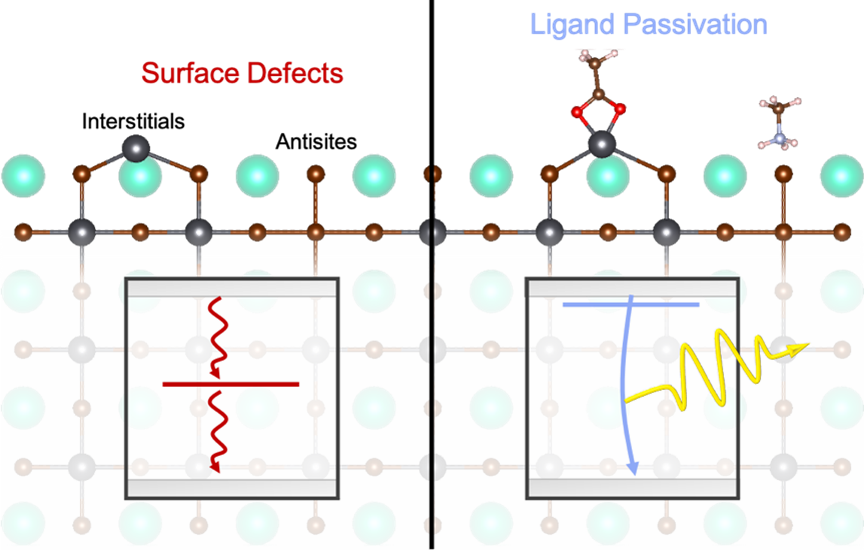
\includegraphics{figures/defect_passivation.png}
    \caption{
        Schematic atomic structure of defects at the surface of CsPbBr$_3$, which are susceptible to non-radiative recombination when unpassivated (left), but become less detrimental to radiative recombination when passivated (right).
    }
    \label{fig:defect}
\end{figure}

\textcolor{red}{Descriptions of selected type-B projects.}
\subsubsection{Ultrafast dynamics in strong-field ionized liquid water} 
\begin{figure}[h]
    \centering
    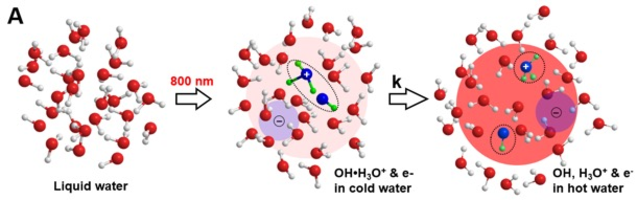
\includegraphics{figures/Water}
    \caption{
        The ionization of liquid water and formation of solvated \(\mathrm{H_3O^+}\), \(\mathrm{OH\cdot}\) radical and electron species is followed by the local thermalization involving energy exchange between the electronic and ionic degrees of freedom.
    }
    \label{fig:water}
\end{figure}

Photo-excitation induced structural dynamics in liquid water represents a paradigmatic case of excited state electron-ion dynamics in the condensed phase. 
In particular, the radiolysis of liquid water and its aftermath is a process of fundamental importance in a variety of technological contexts~\cite{Garrett2005} such energy harvesting, biochemistry, biomedicine, corrosion mitigatio, etc. 
Therefore, investigating the interplay between the electronic and ionic degrees of freedom in photo-ionized liquid water on the femto-picosecond timescales relevant to the creation and transformation of short-lived reaction intermediates~\cite{Loh2020} is of interest to both experiment and theory.
Within the current funding period, NPNEQ researchers at SLAC collaborated with experimental teams working at SLAC's MeV-UED instrument to uncover the structural finger-prints of hydronium cation-hydroxyl radical pairs on femtosecond timescales in strong-field ionized liquid water (See Fig~\ref{fig:water}). 
In this study we deployed velocity-gauge real-time TDDFT as implemented within the \textsc{SALMON} code~\cite{salmon} to estimate the photo-ionization fraction in liquid water for experimentally relevant laser pulse parameters. 
Our simulations revealed a nonlinear multi-step photo-ionization process in liquid water subjected to high-intensity near-infrared radiation and our predicted excited electron energy distribution subsequently informed classical models of thermalization based on molecular dynamics. A manuscript summarizing the findings of our experiment-theory collaboration is currently under review at the journal \textit{Science}.
In the near future we plan to further extend our studies in this prototypical water system by simulating nonadiabatic Ehrenfest electron-ion dynamics during and after laser illumination using our RT-TDDFT platform \textsc{inq} and compare our results with recent ultrafast experiments. 
\subsubsection{WTe2 collaborations}

\subsubsection{Sangeeta's collaborations at the Foundry}
In this experimental collaboration, we perform the first ultrafast investigation of TaTe$_2$, which exhibits unique charge density wave (CDW) and lattice structural order characterised by a transition upon cooling from stripe-like trimer chains into a (3x3) superstructure of trimer clusters. 

We develop computational models of the ultrafast photoinduced dynamics in TaTe2. These models will incorporate the electronic and atomic structure as well as their strong interactions to calculate the atomic trajectories. Density-functional calculations indicate that the initial quench is triggered by Ta trimer bonding to nonbonding transitions that destabilises the clusters, unlike CDW melting in other TaX$_2$ compounds.
Utilising MeV-scale ultrafast electron diffraction, the TaTe$_2$ structural dynamics is resolved following intense pulsed laser excitation at 1.2 eV. We observe a rapid 1.4 ps melting of the low-temperature ordered state, followed by recovery of the clusters via thermalisation into a hot superstructure persisting for extended times.  Our work paves the way for further exploration and ultimately directed manipulation of the trimer superstructure for novel applications.



\section{Future Work}
\subsection{Code developments}
\subsubsection{Functionality additions to INQ}
\paragraph{Exact exchange and Axc}
\paragraph{Non-collinear magnetism and spin-orbit}
\paragraph{Spiral boundary conditions}

\paragraph{Beyond Ehrenfest dynamics} 
Mention: Electron-phonon development from stopping power.  Figure.

\paragraph{Interfacing INQ with TB codes}

Mention: Modularity of INQ makes scripting obsolete because of high throughput capability. Workflow improvements in INQ.

\subsection{Science Applications}
\subsubsection{Spin dynamics in layered anti-ferromagnets}
Several ongoing projects involving close collaboration between experimental efforts and theory from this team are in progress.

In collaboration with {\bf Tan} and {\bf Pemmaraju}, {\bf Lindenberg} has been investigating the ultrafast dynamical response of two-dimensional antiferromagnetic materials.
In antiferromagnets, electron exchange interactions result in antiparallel or non-collinear microscopic spin correlations with negligible macroscopic magnetization.
Given their low-loss, intrinsic THz frequencies, and insensitivity to stray fields, antiferromagnetic spintronics holds great potential in realizing high-speed communications and new types of information storage technologies. 
Atomically-thin van der Waals crystals like \(\mathrm{FePS_3}\), \(\mathrm{NiPS_3}\) and \(\mathrm{MnPS_3}\) represent a new type of antiferromagnetic materials class with strong 2D quantum confinement and the ability to tune this functionality at high speed and with low energy cost taking advantage of the weak interlayer van der Waals bond.
In initial work we have carried out time domain THz emission spectroscopy probing the ultrafast dynamics of the magnetization in exfoliated flakes of \(\mathrm{NiPS_3}\).
In these experiments an ultrafast optical pump pulse excites above band gap at \(400~\mathrm{nm}\) to create free carriers which then couple to the intrinsic magnetization of the material.
By detecting the emitted THz fields from the sample we probe the time-dependent free (associated with the flow of electrons) and bound (associated with the time-dependent magnetization) currents.  Following directly from Maxwell’s equations one finds: 

\begin{equation}
\mathbf{E}_\text{THz} \propto \frac{\partial\mathbf{J}}{\partial t}+ \frac{\partial}{\partial t} (\nabla \times \mathbf{M})
\end{equation}

where \(\mathbf{J}\) is the free current and \(\mathbf{M}\) is magnetization. 
Fig.~1 shows the experimentally measured THz waveform and the peak-to-peak emission amplitude as a function of temperature, showing an enhancement at the Neel temperature.
This demonstrates the sensitivity of the measurement to the intrinsic antiferromagnetic dynamics.
Further, by measuring the polarization state of the emitted THz fields one can extract information about the crystallographic directions of the associated currents.
We find there are two contributions to the measured fields, involving a current normal to the sample surface associated with the separation of electrons and holes at the surface superposed on a bound current likely associated with an induced rotation of the initially in-plane antiferromagnetic magnetization state.
Further spectral analysis of the emitted fields may allow us to extract information about particular magnons associated with the light-induced response.
This work opens up new possibilities for controlling the properties of antiferromagnetic materials on ultrafast time-scales. 
Ongoing work additionally involves upcoming experiments at the SLAC National Accelerator Laboratory Ultrafast Electron Diffraction facility where we will in parallel investigate the correlated structural dynamics under similar photoexcitation conditions.

\begin{figure}[ht]
    \centering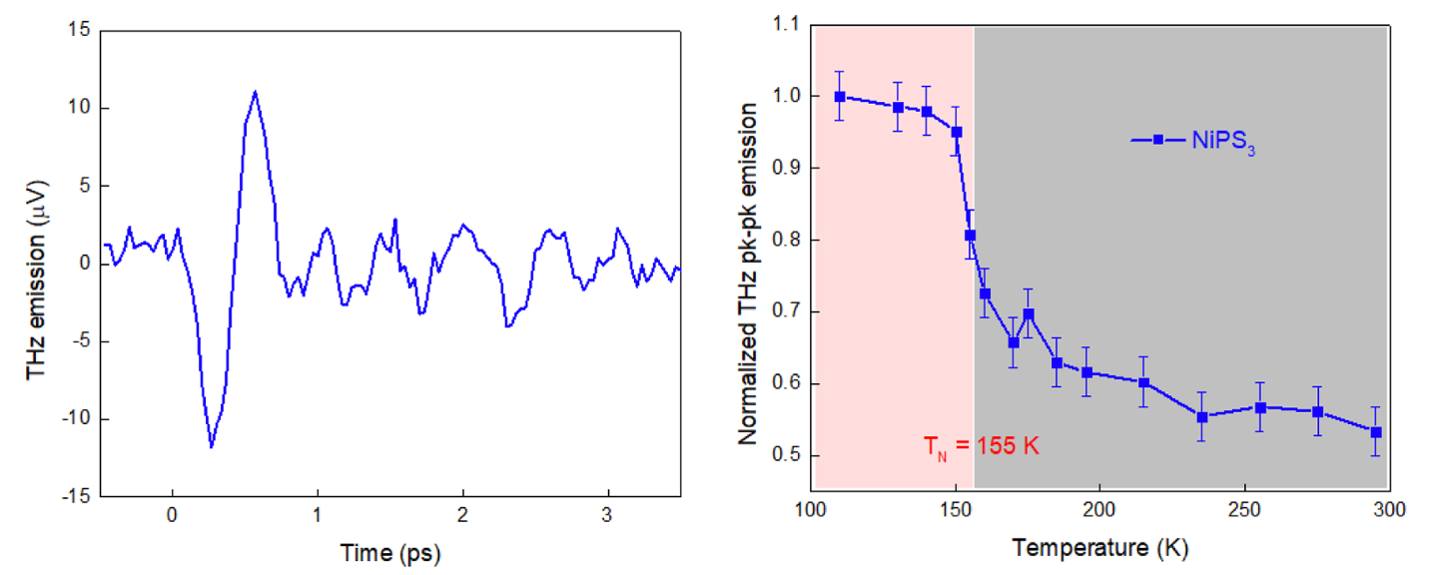
\includegraphics[width=1.0\linewidth]{figures/NiPS3}
    \caption{
        (left)  Measured THz electric field waveform emitted from NiPS3 antiferromagnetic sample under femtosecond \(400~\mathrm{nm}\) excitation.
        (right) Peak THz emission amplitude as a function of temperature, showing strong enhancement at the Neel temperature (\(155~\mathrm{K}\)), showing direct sensitivity to time-dependent magnetization.
    }
    \label{fig:NiPS3}
\end{figure}

In conjunction with this experimental work, {\bf Tan} and {\bf Pemmaraju} are investigating a number of theoretical approaches to this problem.
First, static, first-principles density functional theory are used to solve for the electronic structure, phononic properties, and electron-phonon interactions of the \(\mathrm{NiPS_3}\) materials system. 
Second, the RT-TDDFT approach will be used to directly simulate density and spin fluctuations in time using the INQ code.
The evolution of the calculated diffraction intensities of the spin, charge and orbital patterns will provide dynamics of the order parameters to assist the experimental time-resolved diffraction study.
Trajectories will be examined to understand the structural and electronic mechanisms behind the evolution of spin order peaks, and their associated time scales. 
Finally, the RT-TDDFT simulations will provide data for parameterization of a model for long-wavelength magnon simulations. 
This semi-classical approach involves the construction of an effective spin Hamiltonian consisting of Zeeman, exchange and anisotropic magnetic interactions, with parameters extracted from the INQ code. 
This Hamiltonian will be solved for large magnetic supercell to produce the spin-wave dispersions. 
Development of this model will be accelerated by the team’s recent experience with similar models for 2D TMDCs and manganites~\cite{Siddiqui2020, Rajpurohit2020}. 
As a by-product of this work, the \textsc{inq} code will contain an interface that will facilitate user extraction of parameters for model simulations.

\subsubsection{Halide Perovskites/Photovoltaics/Exciton dynamics}

\subsubsection{Nonlinear nonequilbrium response in topological materials}

Nonlinear optical phenomena arise when light at sufficiently high intensities interacts with matter. Nonlinear response underlies technologically important physical effects including shift-currents, harmonic generation and frequency upconversion in photovoltaic and optoelectronics applications among others.  Recent insights that nonlinear responses are intimately tied to the fundamental topological properties of the quantum materials, has added to the interest in controlling the excited states of these systems with  ultrafast pump-probe and nonlinear multidimensional spectroscopies.

The computational studies proposed in this project are inspired by recent joint experiment-theory results reported by PIs Lindenberg and Pemmaraju on ultrafast nonlinear responses in the Weyl semimetal WTe$_2$ . Our studies showed that terahertz frequency light pulses induce large amplitude interlayer shear strains in WTe$_2$ , modulating its symmetry and potentially its topological phase. The THz induced shear strains in WTe were also found to be associated with a large transient modulation of the second harmonic generation (SHG) response whereby in the THz driven sample, the SHG response is dramatically reduced compared to noncentrosymmetic bulk WTe However since the low order nonlinear response in materials is fundamentally connected with topological quantities such as the Berry connection and Berry curvature , the question remains as to whether the observed transient reduction in SHG is a signature of a topological phase transition involving the annihilation of Weyl nodes in the Bloch band structure or that of a structural transition to a centrosymmetric geometry.

We will investigate the electronic vs structural origins of recently observed large transient changes in the second harmonic response of the Weyl semimetal WTe$_2$ in response to terahertz driven lattice modulations. The relationship between symmetry, topology and SHG response in WTe$_2$ will be investigated using both frequency and time-domain approaches. Simulations of SHG response in \textsc{inq} will go beyond the Born-Oppenheimer approximation to model intrinsic non-equilibrium states involving transient field-driven modulations of the electrons and holes near the Weyl band crossing points. Utilizing the Ehrenfest dynamics capability of the \textsc{inq} code, we plan to investigate the role of transient in-plane currents in driving the observed 0.24 THz shear-shear responses in WTe$_2$, and the role of electron doping in tuning these responses. Such studies will contribute significantly to a detailed material specific understanding of ultrafast nonlinear response in topological materials within the TMDC family and beyond.

\clearpage
